\chapter{Problem Statement}




{\color{red} Esta muy floja esta parte, siga escribiendo basese de buenas referencias, por ejemplo el capítulo 13 de (Planning algorithms- Steven M. LaValle) particularmente 13.1.2 Kinematics for Wheeled Systems }







\section{Vehicle Modelling}


\subsection{Particle Model}
\subsection{Linear Model}
\subsection{Nonlinear Model}



\section{Automated driving}
The main idea in automated driving is to achieve coordination and synchronization of a number of autonomous vehicles (AV), in a safe and efficient way.\\

To manage a huge number of  AV requires a large network with high computational loads, and advanced control techniques. In the literature, is usually implemented one action control for an agent. However, automated driving is an area that must take into account different scenarios and situations. Besides, it is important to prove all possibilities for warranty security and entirely controllability. In this thesis, we study the different control theories and which is the best state to implement. 
\begin{itemize}
    \item  \textbf{Data-enabled Predictive Control:} where is a predictive control that uses past motion data of Vehicle to estimate the future states.
    \item  \textbf{Mixed-Integer Potential Game:} where uses integer and continuous variables in the cost function to control the AV's position and velocity on a highway in an optimal way.
    \item  \textbf{Alternating Direction Method of Multipliers:} where the use of linear model of the AV and some inequality constraints is possible to get a faster and efficient solution of the problem. With this theory is possible to manage a swarm of AV in a decentralized framework
\end{itemize}

All the above controllers are explained in chapter 4. In addition, the next section is explained how the AV and the collision avoidance are modeled. 

\section{Kinematics Model}
We use a unicycle model to represent the kinematics of each vehicle \cite{kinematic}. This model is usually described by a simple non/linear model: 


\begin{equation}
\begin{align*}
  \dot{x} =& v \cos{\theta}\\ 
  \dot{y} =& v \sin{\theta} \\
\dot{\theta} =& \omega  \\ 
\dot{v} =& \frac{R}{2m} (F_{r} + F_{l}) \\ 
\dot{\omega} =& \frac{R}{L \cdot I} (F_{r} - F_{l})  \\ 
\end{align*}
\end{equation}

where $x,y$ are the position in the map and $\theta$ correspond to the orientation in the world reference. Let $v, w$ be the linear and angular velocity inputs, respectively. In Fig. \ref{kinematic2} is possible to see the representation of the mentioned variables


\begin{figure}
\begin{center}
    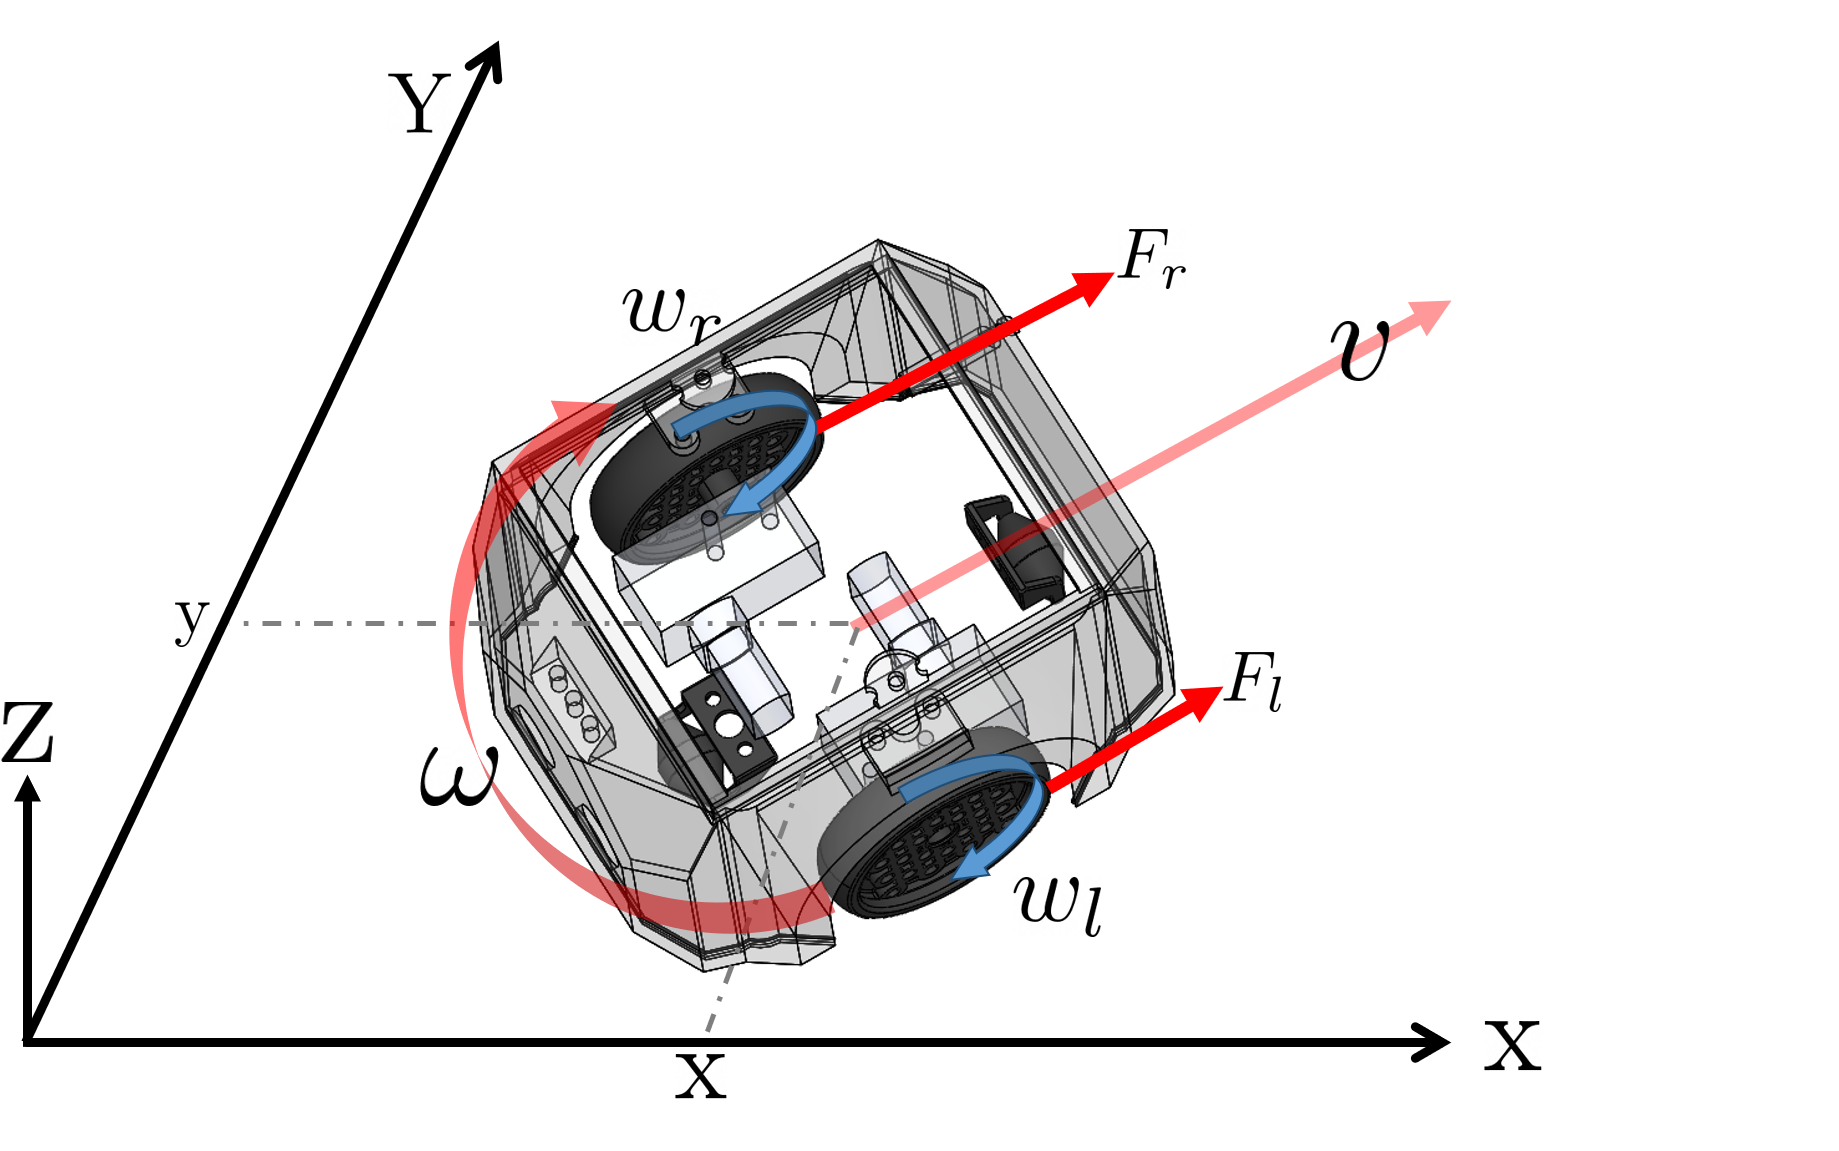
\includegraphics[width=0.8\textwidth]{Kap3/kinematic.png}
    \caption{Kinematic model of a differential robot.}
    \label{kinematic2}
\end{center}
\end{figure}


\begin{equation}
\begin{bmatrix}
w_{r}\\ w_{l}
\end{bmatrix} =  \frac{1}{2R}\begin{bmatrix}
2 & -L\\ 
2 & L
\end{bmatrix} \begin{bmatrix}
v\\ w
\end{bmatrix}.
\label{dif_equat}
\end{equation}

The robot uses a differential model in the low-level control architecture. This model allows calculating the control action in each wheel. In equation \eqref{dif_equat}, it is possible to see the math calculus to obtain the wheel velocity, where $w_{r}$ and $w_{l}$ are angular velocity of right and left wheels, respectively $L$ is the distance between the two wheels, and $R$ is the radius of both wheels. 







\section{Collision Avoidance Modelling}